% Options for packages loaded elsewhere
\PassOptionsToPackage{unicode}{hyperref}
\PassOptionsToPackage{hyphens}{url}
%
\documentclass[
  14pt,
]{extarticle}
\usepackage{amsmath,amssymb}
\usepackage{lmodern}
\usepackage{iftex}
\ifPDFTeX
  \usepackage[T1]{fontenc}
  \usepackage[utf8]{inputenc}
  \usepackage{textcomp} % provide euro and other symbols
\else % if luatex or xetex
  \usepackage{unicode-math}
  \defaultfontfeatures{Scale=MatchLowercase}
  \defaultfontfeatures[\rmfamily]{Ligatures=TeX,Scale=1}
\fi
% Use upquote if available, for straight quotes in verbatim environments
\IfFileExists{upquote.sty}{\usepackage{upquote}}{}
\IfFileExists{microtype.sty}{% use microtype if available
  \usepackage[]{microtype}
  \UseMicrotypeSet[protrusion]{basicmath} % disable protrusion for tt fonts
}{}
\makeatletter
\@ifundefined{KOMAClassName}{% if non-KOMA class
  \IfFileExists{parskip.sty}{%
    \usepackage{parskip}
  }{% else
    \setlength{\parindent}{0pt}
    \setlength{\parskip}{6pt plus 2pt minus 1pt}}
}{% if KOMA class
  \KOMAoptions{parskip=half}}
\makeatother
\usepackage{xcolor}
\usepackage[margin=1.5cm,bottom=2.5cm,top=2.5cm,headsep=0cm,headheight=5cm]{geometry}
\usepackage{longtable,booktabs,array}
\usepackage{calc} % for calculating minipage widths
% Correct order of tables after \paragraph or \subparagraph
\usepackage{etoolbox}
\makeatletter
\patchcmd\longtable{\par}{\if@noskipsec\mbox{}\fi\par}{}{}
\makeatother
% Allow footnotes in longtable head/foot
\IfFileExists{footnotehyper.sty}{\usepackage{footnotehyper}}{\usepackage{footnote}}
\makesavenoteenv{longtable}
\usepackage{graphicx}
\makeatletter
\def\maxwidth{\ifdim\Gin@nat@width>\linewidth\linewidth\else\Gin@nat@width\fi}
\def\maxheight{\ifdim\Gin@nat@height>\textheight\textheight\else\Gin@nat@height\fi}
\makeatother
% Scale images if necessary, so that they will not overflow the page
% margins by default, and it is still possible to overwrite the defaults
% using explicit options in \includegraphics[width, height, ...]{}
\setkeys{Gin}{width=\maxwidth,height=\maxheight,keepaspectratio}
% Set default figure placement to htbp
\makeatletter
\def\fps@figure{htbp}
\makeatother
\setlength{\emergencystretch}{3em} % prevent overfull lines
\providecommand{\tightlist}{%
  \setlength{\itemsep}{0pt}\setlength{\parskip}{0pt}}
\setcounter{secnumdepth}{-\maxdimen} % remove section numbering

\usepackage{gensymb}
\usepackage{mhchem}
\usepackage{tcolorbox}
\usepackage{fancyhdr}
\usepackage{graphicx}
\usepackage{titling}
\ifLuaTeX
  \usepackage{selnolig}  % disable illegal ligatures
\fi
\IfFileExists{bookmark.sty}{\usepackage{bookmark}}{\usepackage{hyperref}}
\IfFileExists{xurl.sty}{\usepackage{xurl}}{} % add URL line breaks if available
\urlstyle{same} % disable monospaced font for URLs
\hypersetup{
  pdftitle={Chemical Measurements},
  hidelinks,
  pdfcreator={LaTeX via pandoc}}

\title{\textbf{Chemical Measurements}}
\usepackage{etoolbox}
\makeatletter
\providecommand{\subtitle}[1]{% add subtitle to \maketitle
  \apptocmd{\@title}{\par {\large #1 \par}}{}{}
}
\makeatother
\subtitle{\textbf{Unit 1:} Some Basic Concepts in Chemistry}
\author{}
\date{}


\pagestyle{fancy}
% \graphicspath{{./images/}}
\fancyhead[C]{
\includegraphics[width=2cm]{./images/fplogo}}
\fancyhead[L]{JEE Chemistry\\~\\}
\fancyhead[R]{\thetitle{}\\~\\}
\renewcommand{\headrulewidth}{0pt}
\renewcommand{\footrulewidth}{2pt}
\newtcolorbox{myquote}{colback=gray!25, colframe=gray!75!black}
\renewenvironment{quote}{\begin{myquote}}{\end{myquote}}
% \let\OldRule\rule
% \renewcommand{\rule}[2]{\OldRule{\linewidth}{#2}}

\begin{document}
\maketitle
\thispagestyle{fancy}

\begin{quote}
\textbf{Topics:} Physical quantities and their measurements in
Chemistry; Precision and Accuracy; Significant Figures; SI Units;
Dimensional Analysis
\end{quote}

\hypertarget{properties-of-matter}{%
\section{Properties of Matter}\label{properties-of-matter}}

All substances have various characteristic properties. These properties
can be physical or chemical.

\textbf{Physical properties} can be measured/observed without changing
the identity of a substance. (\emph{Eg: Color, Mass, Melting and Boiling
Point})

On the other hand, the measurement of \textbf{Chemical properties}
require the occurence of a chemical change. (\emph{Eg: Acidity,
Basicity, Combustibility})

\hypertarget{measuring-physical-properties}{%
\section{Measuring Physical
Properties}\label{measuring-physical-properties}}

Physical properties such as mass, length, volume, etc. are quantitative
in nature, and are expressed by a number followed by units.

\[{47~\mathrm{km}}\]

\hypertarget{si-units}{%
\section{SI Units}\label{si-units}}

By convention, scientists use the \textbf{SI System of Units} as a
standard for measurement of various physical properties.

In the SI system, units for \textbf{seven} base quantities are defined.
(See Figure 1.) All the other quantities can be derived by from the base
quantities.

\begin{figure}
\centering
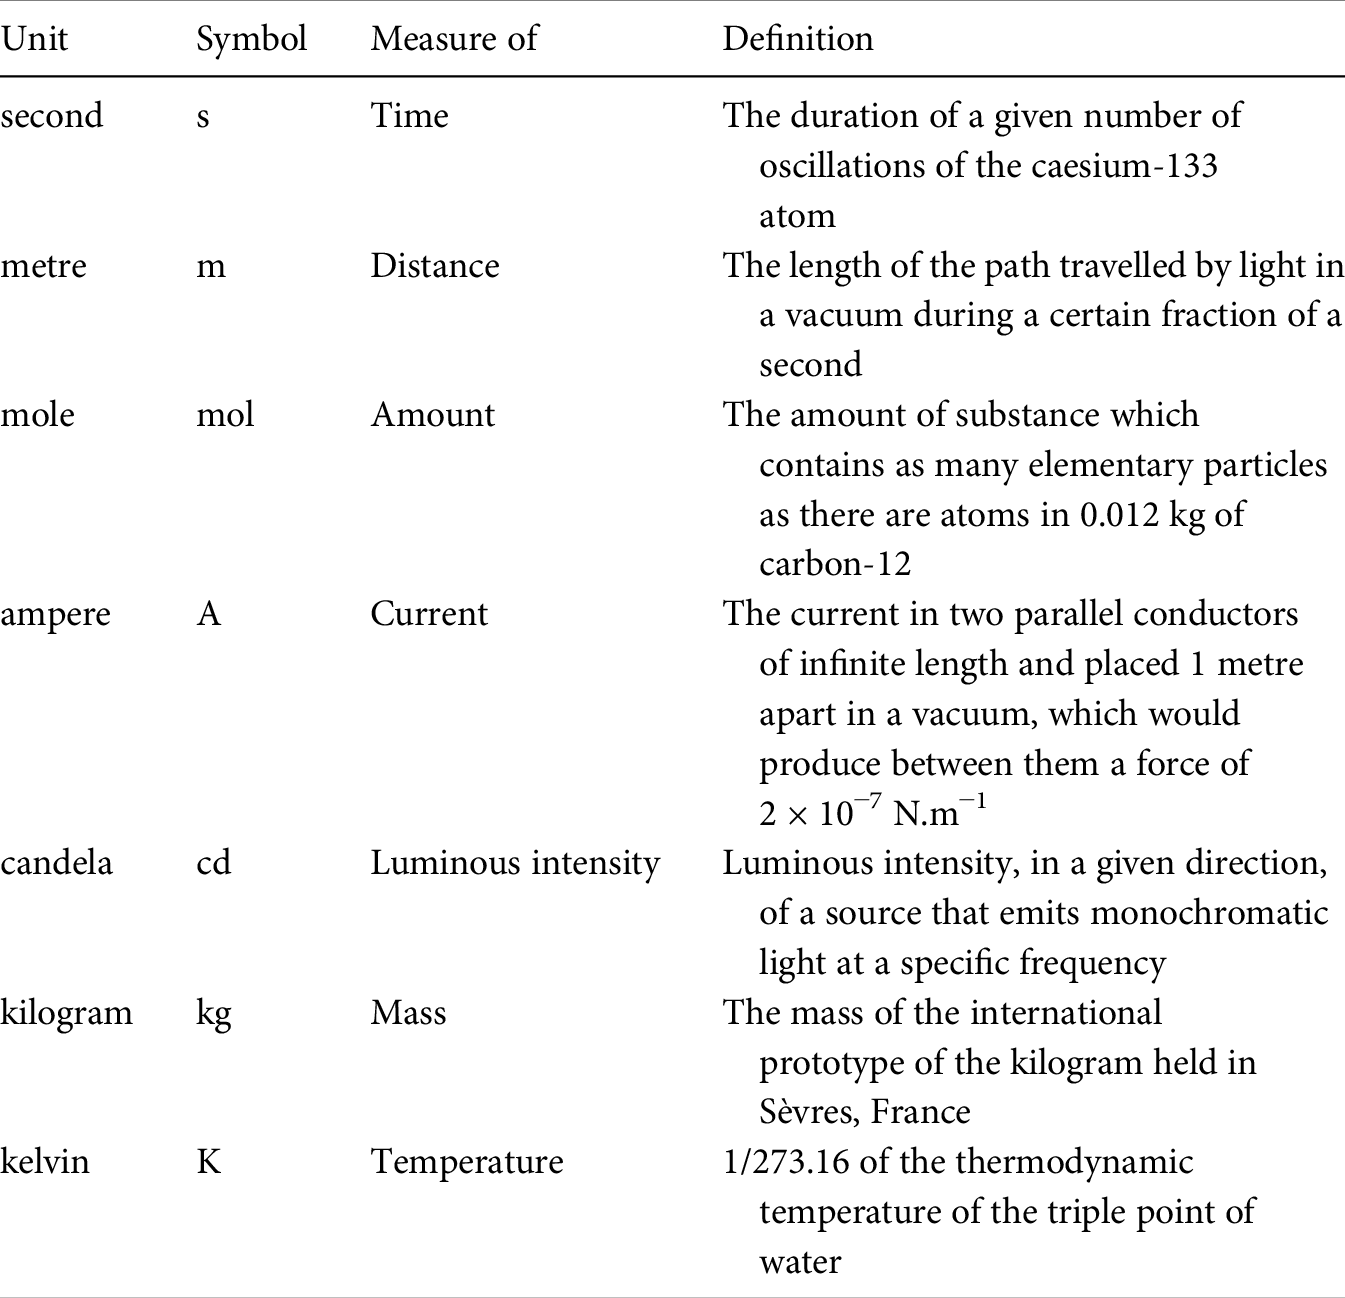
\includegraphics{./images/2022-06-12-22-49-50.png}
\caption{Definition of SI Base units}
\end{figure}

\begin{quote}
\textbf{Derived Units}

SI Units for quantities such as speed, force, energy can be derived from
the seven base units.
\[{\mathrm{Speed:}\mkern3mu \mathrm{m}\mkern3mu \mathrm{s^{-1}}}\]
\[{\mathrm{Force:}\mkern3mu \mathrm{kg}\mkern3mu \mathrm{m}\mkern3mu \mathrm{s^{-2}}}\]
\[{\mathrm{Energy:}\mkern3mu \mathrm{kg}\mkern3mu \mathrm{m^{2}}\mkern3mu \mathrm{s^{-2}}}\]
\end{quote}

\hypertarget{common-prefixes}{%
\subsection{Common prefixes}\label{common-prefixes}}

These prefixes are used with the SI units to express a large or small
quantities.

\begin{longtable}[]{@{}ccc@{}}
\toprule()
\textbf{Multiple} & \textbf{Prefix} & \textbf{Symbol} \\
\midrule()
\endhead
\(10^{-15}\) & femto & \({\mathrm{f}}\) \\
\(10^{-12}\) & pico & \({\mathrm{p}}\) \\
\(10^{-9}\) & nano & \({\mathrm{n}}\) \\
\(10^{-6}\) & micro & \({\mathrm{\mu}}\) \\
\(10^{-3}\) & milli & \({\mathrm{m}}\) \\
\(10^{3}\) & kilo & \({\mathrm{k}}\) \\
\(10^{6}\) & mega & \({\mathrm{M}}\) \\
\(10^{9}\) & giga & \({\mathrm{G}}\) \\
\(10^{12}\) & tera & \({\mathrm{T}}\) \\
\bottomrule()
\end{longtable}

\hypertarget{physical-properties}{%
\section{Physical Properties}\label{physical-properties}}

\hypertarget{mass}{%
\subsection{Mass}\label{mass}}

In the SI system, mass is measured in \({\mathrm{kg}}\). However, in a
laboratory, \({\mathrm{g}}\) is used due to small amounts of chemicals
used.

\begin{quote}
In chemistry, the terms `weight' and `mass' are often interchangably
used.
\end{quote}

\hypertarget{volume}{%
\subsection{Volume}\label{volume}}

The SI unit of volume is \(\mathbf{{\mathrm{m^{3}}}}\). In a chemical
laboratory, \(\mathbf{{\mathrm{cm^{3}}}}\) or
\(\mathbf{{\mathrm{dm^{3}}}}\) is often used.

A common unit of volume is \(l\), which is used for measurement of
volume of liquids.

\[{1~\mathrm{\textit{l}~}\mkern3mu \mathrm{=}\mkern3mu \mathrm{1}\mkern3mu \mathrm{dm^{3}}\mkern3mu \mathrm{=}\mkern3mu \mathrm{1000}\mkern3mu \mathrm{cm^{3}}}\]

The volumes of liquids can be measured using laboratory devices like
\textbf{burette}, \textbf{pipette}, and \textbf{graduated cylinder}.

\hypertarget{density}{%
\subsection{Density}\label{density}}

Density refers to the amount of mass of a substance per unit volume. If
density is more,
\(\text{\underline{it means particles are more closely packed}}\).

\[{\mathrm{Density}\mkern3mu \mathrm{=}\mkern3mu \mathrm{\frac{Mass}{Volume}}}\]

\[{\mathrm{SI}\mkern3mu \mathrm{unit}\mkern3mu \mathrm{of}\mkern3mu \mathrm{density\rightarrow kg}\mkern3mu \mathrm{m^{-3}}}\]

In a lab, density is often expressed in
\({\mathrm{g}\mkern3mu \mathrm{cm^{-3}}}\)

\hypertarget{temperature}{%
\subsection{Temperature}\label{temperature}}

The SI Unit of temperature is Kelvin (\({\mathrm{K}}\)). However, around
the world people use \({\mathrm{{}^{\circ}C}}\) and
\({\mathrm{{}^{\circ}F}}\) to measure temperature.

\[{\mathrm{{}^{\circ}F=\frac{9}{5}({}^{\circ}C)}\mkern3mu \mkern3mu \mkern3mu \mathrm{32}}\]
\[{\mathrm{K={}^{\circ}C}\mkern3mu \mkern3mu \mkern3mu \mathrm{273.15}}\]

\begin{quote}
In the Kelvin scale, the temperature \({0~\mathrm{K}}\) is referred to
as the \(\textbf{absolute zero}\), as it is the minimum temperature
possible.
\end{quote}

\begin{longtable}[]{@{}cccc@{}}
\toprule()
\textbf{Scale} & \textbf{Water Freezing} & \textbf{Water Boiling} &
\textbf{Room Temperature} \\
\midrule()
\endhead
\({\mathrm{{}^{\circ}C}}\) & \({0~\mathrm{{}^{\circ}C}}\) &
\({100~\mathrm{{}^{\circ}C}}\) & \({25~\mathrm{{}^{\circ}C}}\) \\
\({\mathrm{{}^{\circ}F}}\) & \({32~\mathrm{{}^{\circ}F}}\) &
\({212~\mathrm{{}^{\circ}F}}\) & \({77~\mathrm{{}^{\circ}F}}\) \\
\({\mathrm{K}}\) & \({273.15~\mathrm{K}}\) & \({373~\mathrm{K}}\) &
\({298~\mathrm{K}}\) \\
\bottomrule()
\end{longtable}

\hypertarget{scientific-notation}{%
\section{Scientific Notation}\label{scientific-notation}}

To express very large or very small numbers, we use
\(\text{\underline{scientific notation}}\).

Here, the number is expressed as a product of \(N\) and \(10^n\) where
\(N\) is a number from 1 to 10 (not including 10), and \(n\) is any
integer.

\[N\times 10^n\tag{$0\le N<10$; $n\in \mathbb{Z}$}\]

\[0.00016={1.6\times 10^{-4}}\]
\[232.508={2.325\mkern2mu 08\times 10^{2}}\] \[200000={2\times 10^{5}}\]

\begin{quote}
\begin{itemize}
\tightlist
\item
  The exponent is equal to the number of places the decimal point was
  shifted.
\item
  If the point is shifted to the right (the number is increased), then
  the exponent is negative. (and vice versa)
\end{itemize}
\end{quote}

\begin{quote}
\textbf{Operations on numbers in Scientific Notation}

\begin{itemize}
\item
  \textbf{Multiplication and Division}: Numbers can be directly
  multiplied when in scientific notation. Here, the exponents
  add/subtract accordingly.
  \[({1.6\times 10^{9}})\times({6.9\times 10^{-3}})\]
  \[=1.6\times 6.9\times 10^{6}\] \[=11.04\times 10^{6}\]
\item
  \textbf{Addition and Subtraction}: We need to convert both the numbers
  to have the same exponent in order to add or subtract them.
  \[({1.6\times 10^{9}}) ({6.4\times 10^{8}})\]
  \[({16\times 10^{8}}) ({6.4\times 10^{8}})\] \[22.4\times 10^8\]
\end{itemize}
\end{quote}

\hypertarget{rounding-off-results}{%
\section{Rounding Off Results}\label{rounding-off-results}}

Often, we will need to round off numbers to indicate the amount of
precision in the answer. (In this section, all numbers are rounded off
to the nearest tenths as an example.)

\textbf{Steps to round off a number}

\begin{itemize}
\item
  If the digit to be removed is more than 5, the preceding number is
  increased by 1. \[32.47\rightarrow 32.5\]
\item
  If the digit to be removed is less than 5, the preceding number is not
  changed. \[32.43\rightarrow 32.4\]
\item
  If the digit to be removed is 5, then:

  \begin{itemize}
  \tightlist
  \item
    the preceding number is not changed if it is even.
  \item
    the preceding number is increased by 1 if it is odd.
    \[32.45\rightarrow 32.4\] \[32.75\rightarrow 32.8\]
  \end{itemize}
\end{itemize}

\begin{quote}
\textbf{Precise and Accurate Measurements}\\
\(\text{\underline{Precision}}\) refers to the closeness of two results
with each other. (\(1.93\) and \(1.95\))\\
\(\text{\underline{Accuracy}}\) refers to the agreement of a result with
the true value. (\(1.99\) and the true value is \(2.00\))
\end{quote}

\hypertarget{significant-figures}{%
\section{Significant Figures}\label{significant-figures}}

Whenever we make a measurement: say \({35.45~\mathrm{g}}\), there is
bound to be some error. Errors in measurement can arise due to a variety
of reasons, primarily due to the capabalities of the measuring device.

For example, lets say you measure the length of an object to be
\({10.3~\mathrm{cm}}\) using a 30 cm ruler. It is important to note that
the least count the ruler is \({0.1~\mathrm{cm}} ={1~\mathrm{mm}}\).
Therefore, it is possible that the actual length of the object is not
actually \({10.3~\mathrm{cm}}\), some value close to (higher or lower
than) \({10.3~\mathrm{cm}}\) which cannot be accurately measured by the
ruler. On measuring the object with a vernier calipers, we find that the
actual length is \({10.3124~\mathrm{cm}}\).

\[\text{Measurement}={10.3~\mathrm{cm}}\]
\[\text{Actual Value}={10.3124~\mathrm{cm}}\]

Here, we observe, that last digit of the measurement, \(3\) uncertain.
On accounting for the error in the measurement, we can write the value
as \({10.3 {}\pm{} 0.1~\mathrm{cm}}\), meaning the \({10}\) is certain,
and the \({3}\) is uncertain.

\textbf{Significant Figures} are \emph{meaningful digits} which include
all the digits which are known with certainty, plus one digit which is
estimated or uncertain. The uncertainity is indicated by the last
significant digit, which is uncertain. Thus, by convention, in the
measurement \({11.46~\mathrm{L}}\), the uncertainity is \(\pm1\) in the
last digit, \(6\).

\hypertarget{determining-significant-figures}{%
\subsection{Determining Significant
Figures}\label{determining-significant-figures}}

\begin{itemize}
\tightlist
\item
  All non-zero digits are significant.

  \begin{itemize}
  \tightlist
  \item
    Eg: \({13.24~\mathrm{mg}}\) has 4 significant figures.
  \end{itemize}
\item
  Zeroes before the first significant digit are insignificant.

  \begin{itemize}
  \tightlist
  \item
    Eg: \({0.057~\mathrm{m}}\) has 2 significant figures.
  \end{itemize}
\item
  Zeroes between two non-zero digits are significant.

  \begin{itemize}
  \tightlist
  \item
    Eg: \({1.02~\mathrm{km}}\) has 3 significant figures.
  \end{itemize}
\item
  Zeroes at the end of the number are significant, if they are at the
  right of the decimal point.

  \begin{itemize}
  \tightlist
  \item
    Eg: \({0.400~\mathrm{g}}\) has 3 significant figures.\footnote{Here,
      \({4.00~\mathrm{g}}\) is different from \({4~\mathrm{g}}\),
      because the two extra zeroes indicate that the measurement is more
      precise, i.e.~\(4\pm 0.01\) rather than \(4\pm 1\). Thus, it has
      more significant figures.}
  \end{itemize}
\item
  Zeroes at the end of the number maybe insignificant when there is no
  decimal point. Otherwise, the uncerainty is ambiguous. (To avoid
  ambiguity, these numbers are better represented in scientific
  notation.)

  \begin{itemize}
  \tightlist
  \item
    Eg: \({100~\mathrm{m}}\): Here, it is not clear whether the
    uncertainty in measurement is 1, 10 or 100. Generally, we assume
    that the 00 in 100 are estimated and do not represent the actual
    measurement. Thus, it has only 1 significant digit.
  \item
    Eg: \(100.\text{ m}\) has 3 significant figures. The decimal point
    indicates that \(100\) is the actual measured value.
  \item
    Eg: \({100.0~\mathrm{m}}\) has 4 significant figures.
  \end{itemize}
\item
  Counting numbers have infinite significant figures. This is because
  there is no error in the measurement.

  \begin{itemize}
  \tightlist
  \item
    Eg: The measurement ``\(30 \text{ eggs}\)'' has \(\infty\)
    significant figures.
  \end{itemize}
\item
  When numbers are written in scientific notation, all digits are
  significant.

  \begin{itemize}
  \tightlist
  \item
    Eg: \(6.022\times 10^{23}\) has 4 significant figures.
  \item
    Eg: \(2.40\times 10^{-5}\) has 3 significant figures.
  \end{itemize}
\end{itemize}

\hypertarget{operations-of-significant-figures}{%
\subsection{Operations of Significant
Figures}\label{operations-of-significant-figures}}

\textbf{Addition and Subtraction}\\
The result cannot have
\(\text{\underline{more digits after the decimal point}}\), than the
original numbers.

\[\begin{aligned}12.11+18.0+1.012 &=31.122 \\&=31.1\end{aligned}\]

Here, since \(18.0\) only has one decimal place, the result should be
reported with only one digit after the decimal point.

\textbf{Multiplication and Division}\\
The result cannot have \(\text{\underline{more significant figures}}\),
than the original numbers.

\[\begin{aligned}12.64\times 0.12 &= 1.5168 \\&=1.5\end{aligned}\]

Here, since \(0.12\) only has two significant figures, the result should
be reported with only two significant figures.

\hypertarget{dimensional-analysis}{%
\section{Dimensional Analysis}\label{dimensional-analysis}}

\textbf{Dimensional Analysis} or the \textbf{Unit Factor Method} is a
method to convert measurements into different units.

Eg: Convert \({2~\mathrm{L}}\) to \({\mathrm{m^{3}}}\).

\begin{align*}
1~\mathrm{L} &= 100~\mathrm{cm^3} \\
\implies 1 &= \frac{1000~\mathrm{cm^3}}{1~\mathrm{L}} \\
1~\mathrm{m^3} &= 10^6~\mathrm{cm^3} \\
\implies 1 &= \frac{1~\mathrm{m^3}}{10^6~\mathrm{cm^3}}
\end{align*}

\begin{align*}
2~\mathrm{L} &= 2~\mathrm{L}\times \frac{1000~\mathrm{cm^3}}{1~\mathrm{L}} \times \frac{1~\mathrm{m^3}}{10^6~\mathrm{cm^3}}\\
2~\mathrm{L} &= 2\times 10^{-3}~\mathrm{m^3}
\end{align*}

Here, fractions such as \(\frac{1000~\mathrm{cm^3}}{1~\mathrm{L}}\) are
known as unit factors, since they are equal to 1. These can be
multiplied to a measurement without changing its value.

\begin{center}\rule{0.5\linewidth}{0.5pt}\end{center}

\hypertarget{questions}{%
\section{Questions}\label{questions}}

\begin{enumerate}
\def\labelenumi{\arabic{enumi}.}
\item
  How many significant figures will be present in the result of this
  calculation? \[\frac{2.5\times 1.25\times 3.5}{2.01}\]
\item
  What is the difference between expressing the weight of a solid as
  \({36.5\times 10^{3}~\mathrm{g}}\) and
  \({36.50\times 10^{3}~\mathrm{g}}\)?
\item
  A student performs a titration with different burettes and finds titre
  values of \({25.2~\mathrm{mL}}\), \({25.25~\mathrm{mL}}\), and
  \({25.0~\mathrm{mL}}\). The number of significant figures in the
  average titre value is \_\_\_\_\_\_\_\_. \textbf{{[}IIT-JEE 2010{]}}
\item
  A measured temperature on Fahrenheit scale is
  \({200~\mathrm{{}^{\circ}F}}\). What will this reading be on celsius
  scale?
\item
  In which of the following numbers all zeros are significant?

  \begin{enumerate}
  \def\labelenumii{(\Alph{enumii})}
  \tightlist
  \item
    0.500
  \item
    30.000
  \item
    0.00030
  \item
    0.0050
  \end{enumerate}
\end{enumerate}

\end{document}